\chapter{Improving the Model}\label{chap:model_improvements}

In this chapter, I address various questions raised by the literature and use the insights from Chapter~\ref{chap:crnn} to improve the \emph{CRNN}. I perform a series of experiments to test improvements to the model, evaluate a selection of models on the test set and perform qualitative analysis of the model's outputs.

Many of these experiments introduce new hyperparameters. I choose these hyperparameters in a greedy fashion and keep them as specified unless stated otherwise. While the assumption of independence between hyperparameters is certainly be wrong, it is computationally infeasible to perform a full hyperparameter search. Selection based on greedy search is the best option available.

\section{Revisiting the Spectrogram}\label{sec:spectrogram-results}

\subsection{Spectrogram Variants}\label{sec:spectrogram-variants}

It is standard practice in ACR to use a CQT as input. However, \citet{20YearsofACR} raise the question of whether the CQT is truly the best choice. They suggest that the pitch-folding of the CQT may distort the harmonic structure of notes. By contrast, \citet{MelodyTranscriptionViaGenerativePreTraining} use a mel-spectrogram in place of a CQT. 

I test four spectrogram variants in Table~\ref{tab:spectrograms}. These include the standard CQT, mel-spectrogram and linear spectrogram. I also calculate a chroma-CQT to test whether the model is using information from multiple octaves better than a hand-crafted algorithm. The chroma-CQT is calculated by summing CQT values across octaves. Spectrogram calculations are all implemented in \texttt{librosa}~\citep{librosa}. I use $216$ bins for the CQT and mel spectrograms and $2048$ fast Fourier transform (FFT) bins for the linear spectrogram with a hop length of $4096$ for all. 

Results show that CQTs are the best choice. This raises questions as to the validity of the conclusions drawn by \citet{MelodyTranscriptionViaGenerativePreTraining}. They claim that their generative features are better than hand-crafted features. However, they only compare to mel-spectrograms which may not perform as well as CQTs for the related task of melody recognition. The CQT is also better the chroma-CQT. We can be confident that the model is using information from multiple octaves more efficiently than the simply summing across octaves.

\begin{table}[h]
    \centering
    \begin{tabular}{lccccc}
        \toprule
        spectrogram & acc & root & third & seventh & mirex \\  
        \midrule
        CQT & \textbf{60.2} & \textbf{78.4} & \textbf{75.3} & \textbf{62.5} & \textbf{79.5} \\
        chroma-CQT & 50.1 & 71.4 & 65.7 & 52.0 & 69.8 \\
        mel & 52.7 & 69.1 & 66.3 & 54.6 & 70.6 \\
        linear & 51.2 & 66.1 & 63.0 & 53.1 & 73.8 \\
        \bottomrule
    \end{tabular}
    \caption{Results for CQT, chroma-CQT, mel and linear spectrograms. The CQT is certainly the best feature. The other all perform similarly on accuracy and \text{mirex}, but the chroma-CQT does comparatively at identifying thirds and sevenths. }\label{tab:spectrograms}
\end{table}

\subsection{Hop Lengths}\label{sec:hop-lengths}

Different hop lengths have been used to calculate the CQT ranging from 512~\cite{ACRLargeVocab1} up to 4096~\citep{StructuredTraining}. In previous experiments I have used a hop length of $4096$ as is used by the authors of \emph{CRNN}~\citep{StructuredTraining}. Shorter frames would reduce the number of transition frames but require more computational cost. If frame lengths are too short, the Fourier transform may not be able to capture the harmonic structure of the audio.

In Table~\ref{tab:hop_lengths}, I test the effect of different hop lengths on the model's performance. I use a CQT with $216$ bins and a hop length of $512$, $1024$, $2048$, $4096$, $8192$ and $16384$. Results indicate that performance is similar for hop lengths of $4096$ and below. Performance suffers for greater hop lengths. While it could be argued that $2048$ does better than $4096$, this difference is small enough that it is not worth the increased computational cost. Models trained with a hop size of $2048$ take at least twice as long to train and evaluate as those trained on a hop size of $4096$.

\begin{table}[h]
    \centering
    \begin{tabular}{lccccc}
        \toprule
        hop length & acc & root & third & seventh & mirex \\  
        \midrule
        512 & 60.1 & 78.3 & \textbf{75.5} & 62.4 & \textbf{80.0} \\
        1024 & 60.2 & \textbf{78.7} & 75.2 & 62.5 & 79.6 \\
        2048 & \textbf{60.3} & 78.5 & 75.2 & \textbf{62.6} & 79.6 \\
        4096 & 60.0 & 78.1 & 75.0 & 62.2 & 79.2 \\
        8192 & 57.9 & 76.2 & 72.9 & 60.1 & 79.3 \\
        16384 & 53.3 & 71.7 & 68.0 & 55.4 & 77.9 \\
        \bottomrule
    \end{tabular}
    \caption{Results over different hop lengths for CQT calculation. Any hop length in the range $512$ to $4096$ has similar performance. For frames that are any longer, performance suffers. This is likely caused by the requirement for the model to assign a single chord class to each frame. The longer the frame, the greater potential there is for multiple chords to be playing during the frame. }\label{tab:hop_lengths}
\end{table}


\section{Decoding}\label{sec:decoding}

As observed in~\ref{sec:smoothness}, \emph{CRNN} predicts $168$ transitions per song as opposed to the $104$ seen in the ground truth data. I implement a decoding step over the frame-wise probability vectors to smooth predicted labels. Common choices for decoding models include a conditional random field (CRF)~\citep{ACRLargeVocab1, BTC} and a hidden Markov model (HMM)~\citep{BalanceRandomForestACR}. 

I first implement a HMM. The HMM treats the frame-wise probabilities as emission probabilities and the chord labels as hidden states. \citet{CQTvsChroma} note that using a transition matrix with homogeneous off-diagonal entries in the transition matrix performs similarly to using a learned transition matrix. I adopt such a transition matrix for this HMM, with a parameter $\beta$ denoting the probability of self-transition and all other transition probabilities equal to $\frac{1-\beta}{C-1}$. Decoding then follows the Viterbi algorithm~\citep{Viterbi} over the summed forward and backward pass.

A plot of the effect of $\beta$ on the model's performance and the number of transitions per song is shown in Figure~\ref{fig:hmm_beta_search}. From this plot we conclude that smoothing has little affect on the performance of the model while successfully reducing the number of transitions per song to that of the true labels. I choose $\beta = 0.15$ for the remainder of experiments as it results in $102$ transitions per song while maintaining high performance. 

\begin{figure}[H]
    \centering
    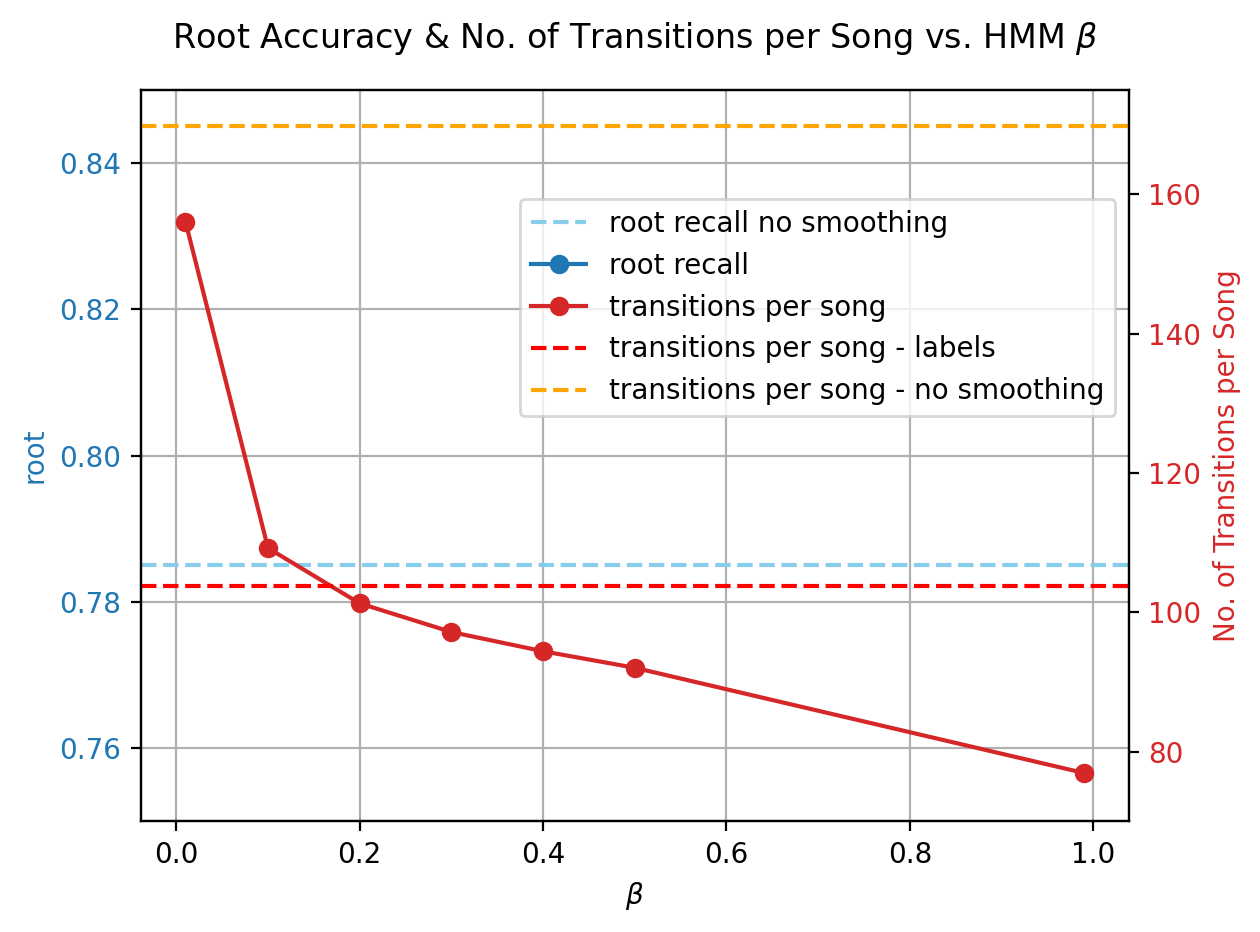
\includegraphics[width=0.8\textwidth]{figures/hmm_beta_vs_root_transitions.png}
    \caption{Effect of the HMM smoothing parameter $\beta$ on the \emph{CRNN} model. As we increase $\beta$, the number of transitions per song decreases. I choose $\beta = 0.15$ as it results in $102$ transitions per song, very close to the $104$ of the ground truth. Performance is stable across $\beta$ with a slight degradation for $\beta > 0.3$. Other performance metrics showed similarly stable results. }\label{fig:hmm_beta_search}
\end{figure}

The effect of the HMM on the incorrect regions previously discussed in Section~\ref{sec:smoothness} can be found in Appendix~\ref{app:histogram_over_region_lengths}. The HMM reduced the percentage of incorrect regions which are a single frame long from $26.7\%$ to $16.7\%$. A more intuitive way to see the effect of the HMM is to look at a section of a song which was the model previously predicted many chord transitions for. This is illustrated in Appendix~\ref{app:hmm_smoothing_effect}.

I also implement a CRF using the \texttt{pytorch-crf} package.\footnote{\url{https://github.com/kmkurn/pytorch-crf}} The CRF is a linear chain CRF with a learned transition matrix.

Results comparing the HMM, CRF and no smoothing can be found in Table~\ref{tab:smoothers}. Both the CRF and HMM reduce the number of transitions per song to a similar level. The HMM outperforms the CRF, with $3.5\%$ greater accuracy. The HMM has almost identical performance to the model with no smoothing. I hypothesise that the learned transition matrix allows the model to overfit to the chord sequences in the training set. Regardless of the explanation, I proceed with HMM smoothing.

\begin{table}[h]
    \centering
    \begin{tabular}{lcccccc}
        \toprule
        smoother & acc & root & third & seventh & mirex & transitions/song\\  
        \midrule
        none & \textbf{60.0} & \textbf{78.1} & \textbf{75.0} & \textbf{62.3} & \textbf{79.2} & 167 \\
        HMM & \textbf{60.0} &\textbf{78.1} & \textbf{75.0} & \textbf{62.3} & \textbf{79.2} & \textbf{102} \\
        CRF & 56.5 & 75.5 & 72.5 & 58.6 & 76.2 & 100 \\
        \bottomrule
    \end{tabular}
    \caption{Results for the HMM and CRF smoothing methods on \emph{CRNN}. The HMM has almost identical performance to the model with no smoothing. However, it drastically reduces the number of transition per song to an acceptable level. The CRF performs notably worse than the HMM. }\label{tab:smoothers}
\end{table}

\section{The Loss Function}

\subsection{Weighted Loss}\label{sec:weighted_loss}

One of the biggest problems with \emph{CRNN} is the low recall on rarer chord qualities. Two common methods for dealing with long-tailed distributions are weighting the loss function and over-sampling. \citet{CurriculumLearning} also explore the use of curriculum learning as form of re-sampling which we do not explore here because they report only minor performance gains. Sampling is explored by \citet{BalanceRandomForestACR} but they use a different model based on pre-computing chroma vectors and re-sampling these chroma vectors for use in training a random forest for frame-wise decoding. 

In our setting, re-sampling training patches of audio may be interesting to explore but is left as future work. It would require a complex sampling scheme as frames cannot be sampled independently. 

Weighting has been explored by \citet{ACRLargeVocab1}. We employ a similar but simpler implementation here. A standard method of weighting is to multiply the loss function by the inverse of frequency of each, with a parameter controlling the strength of the weighting. This is defined in Equation~\ref{eq:weighting}.

\begin{equation}\label{eq:weighting}
    w_c = \frac{1}{{(\text{count}(c) + 10)}^\alpha}
\end{equation}

Where $w_c$ is the weight for chord $c$, $\text{count}(i)$ is the number of frames with chord $c$ in the dataset and $\alpha$ is a hyperparameter controlling the strength of weighting. $\alpha=0$ results in no weighting and increasing $alpha$ increases the severity of weighting. We add $10$ in the denominator to avoid dividing by $0$ and to diminish the dominating effect of chords with very few occurrences. I then define normalised weights $w_c^*$ in Equation~\ref{eq:weighted_loss} so that the learning rate can remain the same.

\begin{equation}\label{eq:weighted_loss}
    w_c^* = \frac{w_c}{s} \text{ where } s = \frac{\sum_{c\in \mathcal{C}} \text{count}(c)\cdot w_c}{\sum_{c\in \mathcal{C}} \text{count}(c)}
\end{equation}

Where $\mathcal{C}$ is the set of all chords in the vocabulary. This keeps the expected weight over samples at $1$ such that the effective learning rate remains the same. These values are calculated over the training set. I test values of $\alpha$ in the set \{0, 0.05, 0.1, \ldots, 0.95, 1\}. The plot in Figure~\ref{fig:weighted_loss} illustrates the effect of the weighting on the model's performance.

\begin{figure}[H]
    \centering
    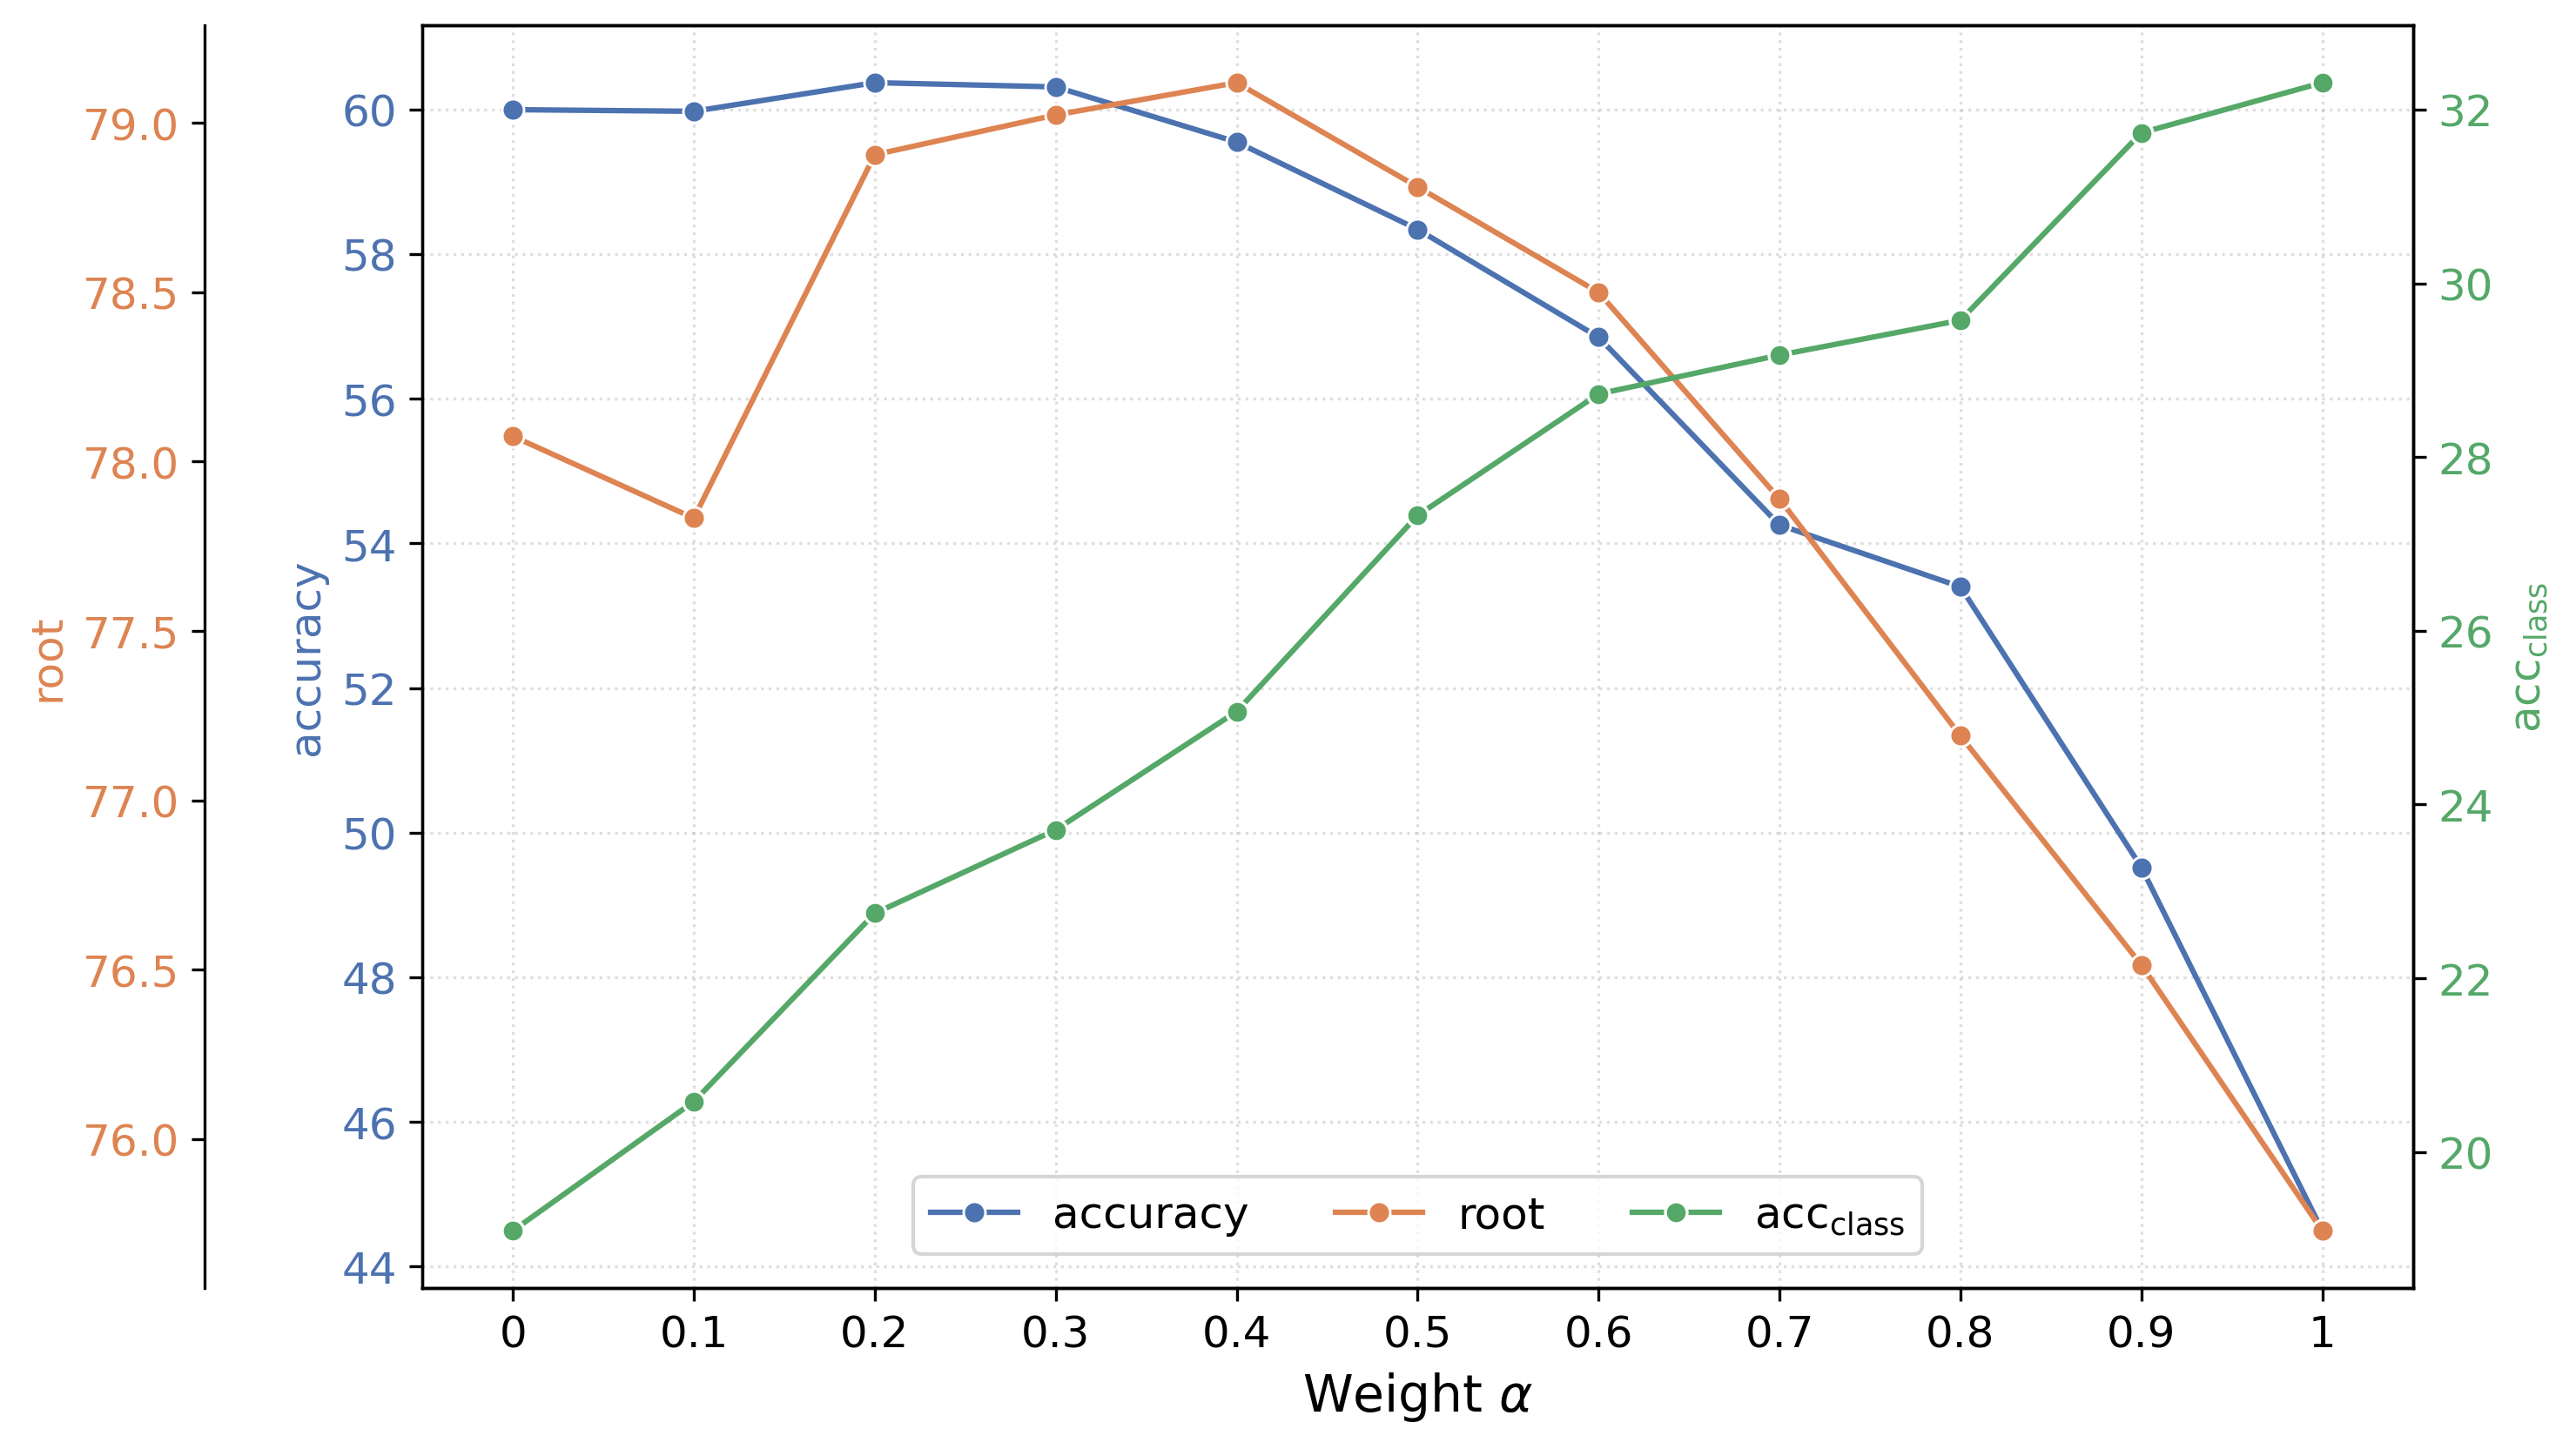
\includegraphics[width=1.0\textwidth]{figures/weight_alpha_search_trim.png}
    \caption{Effect of weighted loss on the \emph{CRNN} model with varying $\alpha$. As we increase $\alpha$, \texttt{acc}\textsubscript{class} improves accuracy and \texttt{root} decrease. I claim there is a sweet-spot where very little overall performance is sacrificed for better class-wise accuracies. I choose this to be $\alpha = 0.3$. The \texttt{root} and \texttt{third} metrics improve and less than $3\%$ is lost on other metrics while mean class-wise accuracy improves by $6\%$ and the median improved by $0.2$. This plot also reveals strong correlation between metrics. }\label{fig:weighted_loss}
\end{figure}

For further insight, a plot of the differences between a confusion matrices with and without weighted loss can be found in Appendix~\ref{app:weighted_loss_confusion_matrix}. Notably, recall on most qualities increases, with recall on major7 doubling to $0.34$. The weighted model predicts $2.2$ times fewer \texttt{X} symbols which may explain how it increases recall on these rarer qualities without sacrificing on accuracy. 

Weighting the loss function also increased the number of transitions predicted per song slightly. This may be because occasional sharp gradient updates cause more extreme probability outputs. I increase the HMM smoothing parameter $\beta$ to $0.2$ to bring the number of transition per song to $104$.

\subsection{Structured Loss}\label{sec:structured_loss}

\citet{StructuredTraining} propose a structured loss function which they claim improves performance on the \emph{CRNN} model. They introduced additional targets of the root, bass and pitch classes. I follow a similar method but do not include the bass as the current chord vocabulary does not consider inversions. The idea behind this loss term is to explicitly task the model with identifying the components of a chord that we care about. This can allow the model to exploit structure in the chord vocabulary such as shared roots and pitch classes, rather than all symbols being predicted independently.

The root can be any of the 12 notes in the Western chromatic scale, \texttt{N} or \texttt{X}, creating a 14-dimensional classification problem. The 12 pitch classes each represent a single binary classification problem. Two fully connected layers calculate a 14-dimensional vector and 12-dimensional vector from the hidden representation outputted from the GRU for the root and pitch classes respectively. Finally, these representations are concatenated with the original output of the model and fed to the final fully connected layer to predict the chord symbol.

The mean cross-entropy loss is calculated in each case. These are then summed to from the \emph{structured loss}. Finally, a linear combination of the structured loss and the original loss is calculated. The final loss is a convex combination of the original loss and the structured loss as defined in Equation~\ref{eq:structured_loss}.

\begin{equation}\label{eq:structured_loss}
    L = \gamma L_{chord} + (1-\gamma)(L_{root} + L_{pitch})
\end{equation}

Where $L$ is the overall loss, $L_{chord}$ is the cross-entropy loss over chords symbols, $L_{root}$ is the cross-entropy loss targeting the root, $L_{pitch}$ is mean binary cross-entropy over each of the pitch classes. $\gamma$ is a hyperparameter controlling the weighting of the original loss. 

The plot in Figure~\ref{fig:structured_loss} illustrates the effect of the structured loss on the model's performance. Choosing $\gamma=0.7$ improves accuracy by $1.3\%$ while \texttt{mirex} worsens by $0.3\%$. Accuracy with \texttt{third} increases by $1.7\%$ and on \texttt{seventh} by $1.3\%$. I keep $\gamma=0.7$ going forward.

\begin{figure}[H]
    \centering
    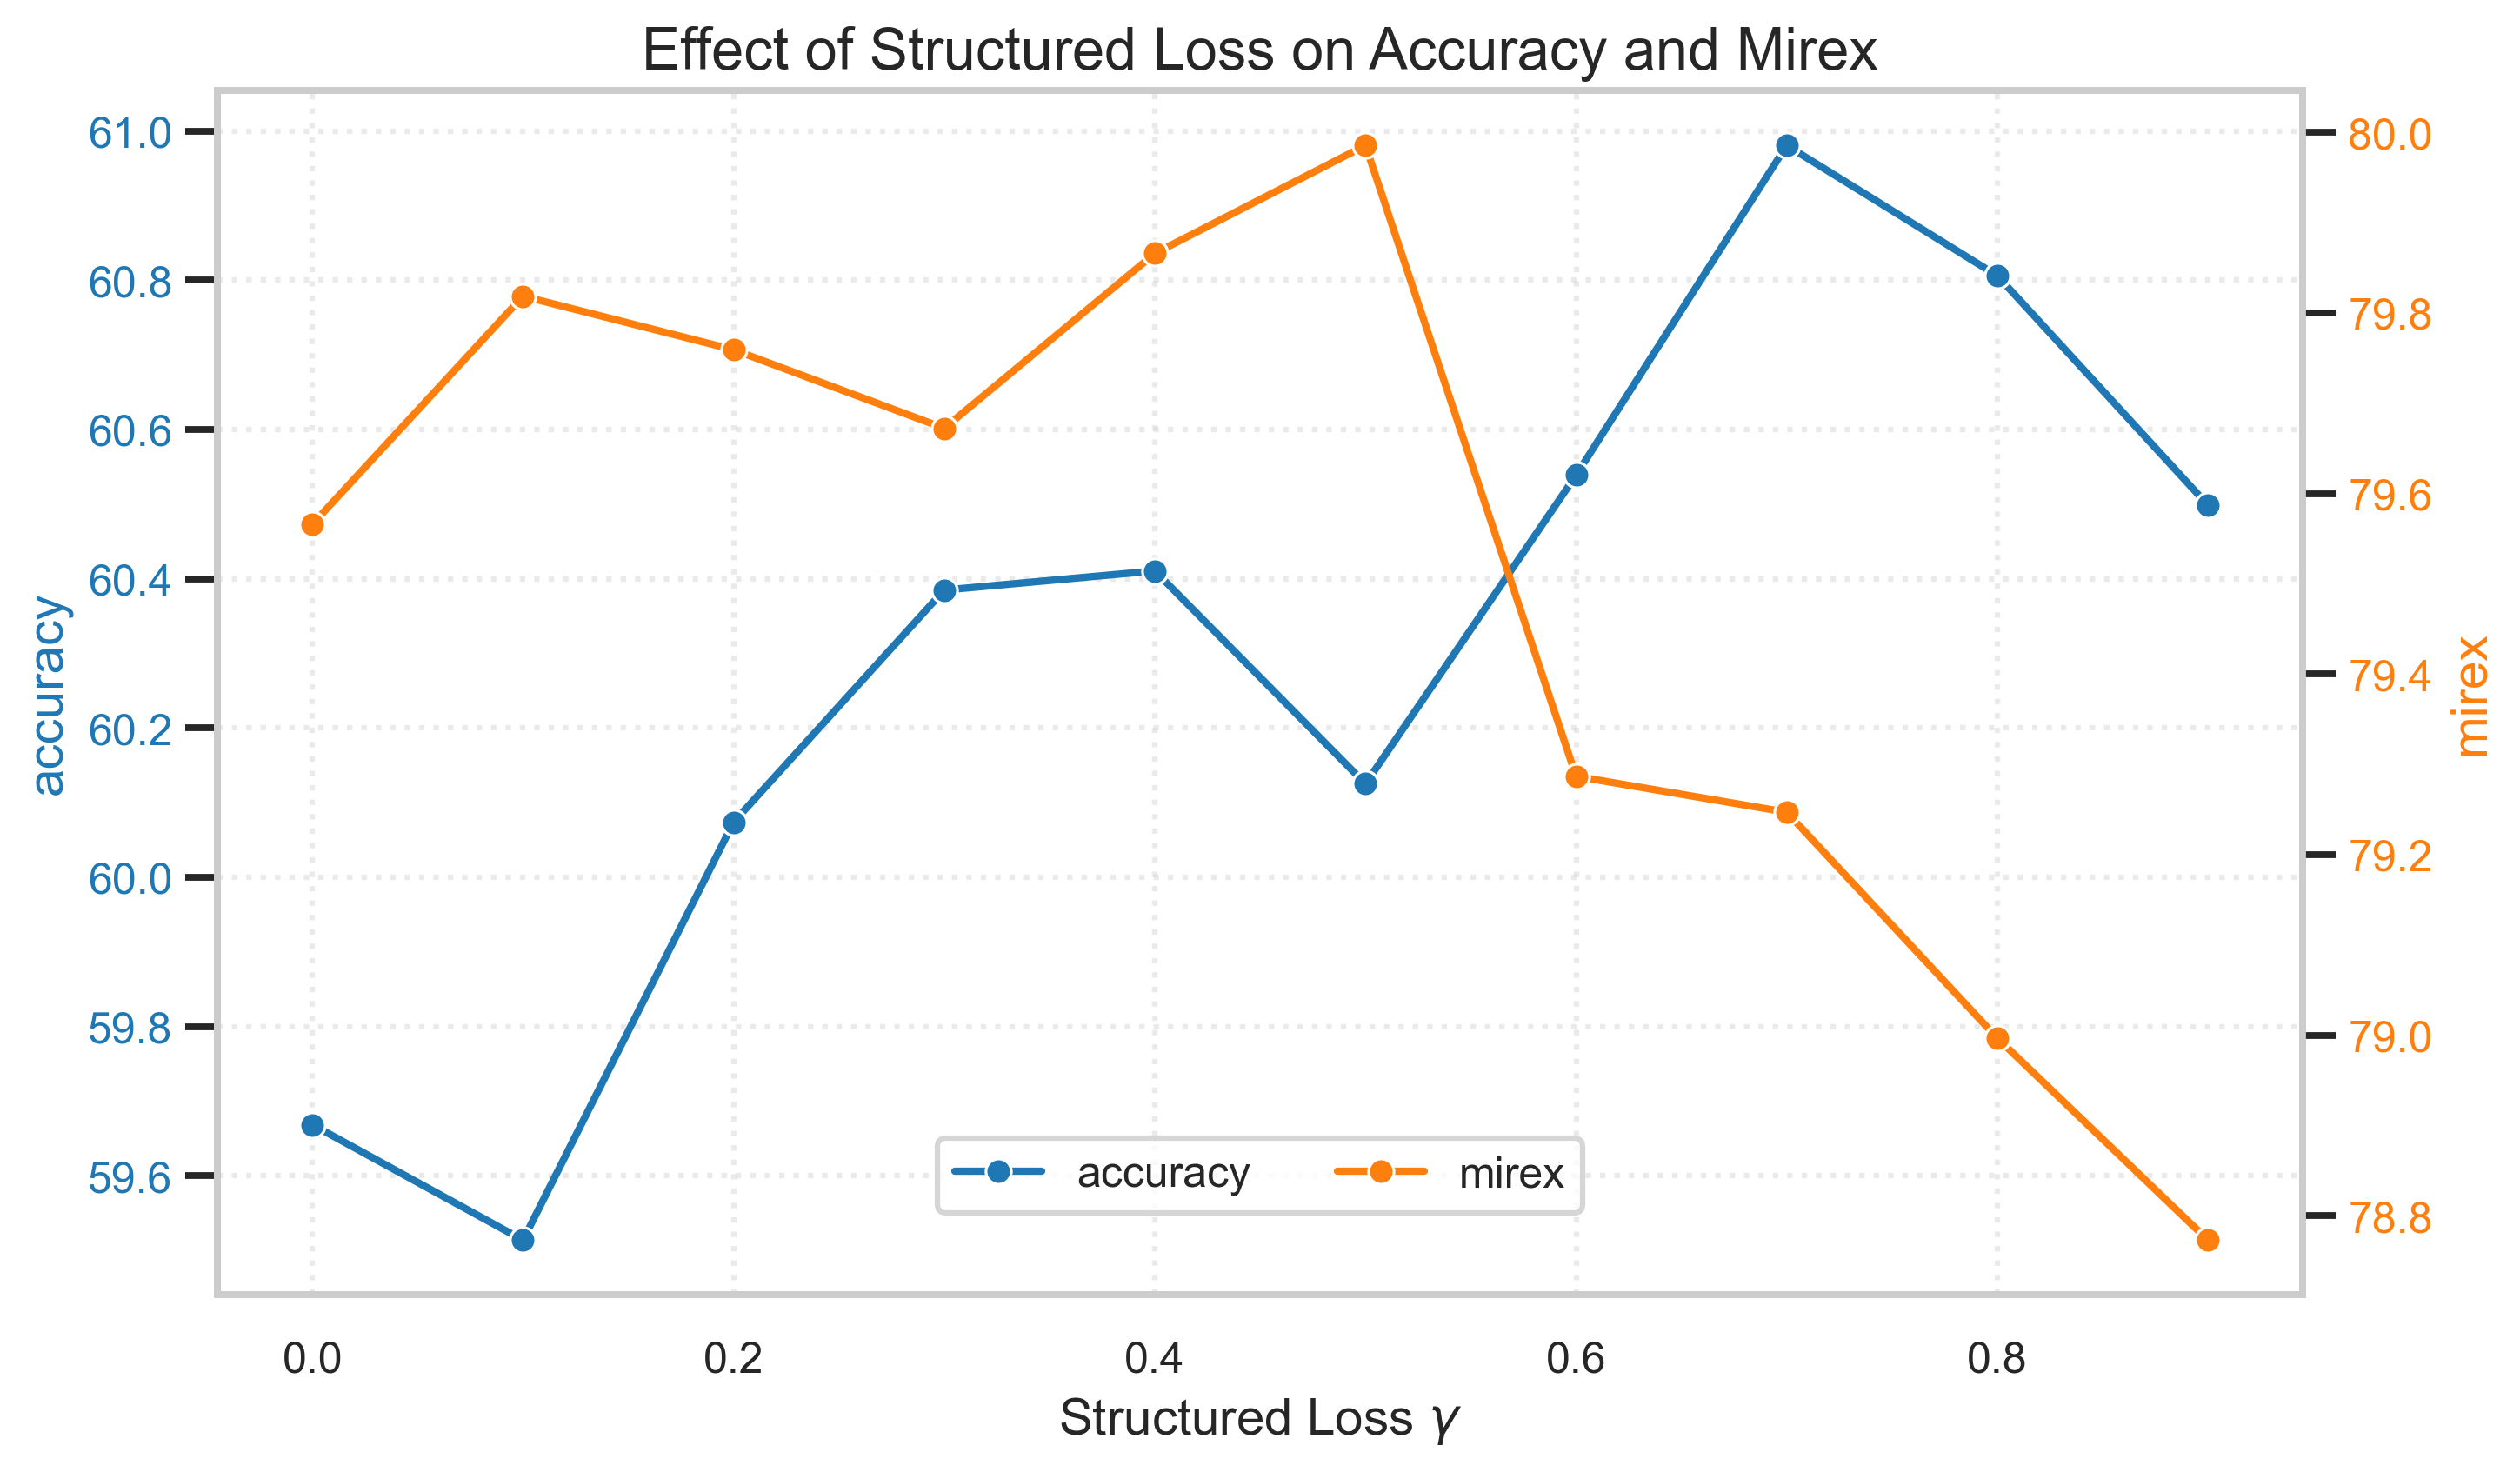
\includegraphics[width=1.0\textwidth]{figures/structured_loss_accuracy.png}
    \caption{Effect of structured loss on the \emph{CRNN} model with varying $\gamma$. As we increase $\gamma$, accuracy improves but \texttt{mirex} behaves erratically, worsening at the higher end. The other metrics behave similarly to accuracy. I choose $\gamma=0.7$ based on peak accuracy. }\label{fig:structured_loss}
\end{figure}

\section{Generative Features}

\citet{MelodyTranscriptionViaGenerativePreTraining} use generative features extracted from Jukebox~\citep{Jukebox} to improve performance for melody transcription. They also produce a chord transcription model using the same methodology but do not report results. I decide to test generative features using MusicGen~\citep{MusicGen} as a feature extractor. This was for several reasons. MusicGen is a newer model. It has several different sizes of model which could be tested against each other as an experiment on the complexity of the model. It has a fine-tuned variant called MusiConGen~\citep{MusiConGen} which is used for synthetic data generation in Section~\ref{sec:synthetic_data}. All model weights are available on the HuggingFace Hub.\footnote{\url{https://huggingface.co/docs/hub/en/index}} Finally, its training data was properly licensed, unlike Jukebox. I leave the results of Jukebox for future work.

\textbf{Feature Extraction}: Overlapping $5$ second chunks of audio were fed through MusicGen in a batched fashion. This first requires passing the audio through the pre-trained Encodec audio tokeniser~\citep{Encodec}. These are then fed through the language model. I take the output logits as the representation for each frame. The model outputs logits in four `codebooks', each $2048$-dimensional vectors, intended to represent different granularities of detail in the audio. Audio segments are overlapped such that every frame has context from both directions. The multiple representations for each frame are averaged. Finally, these representations are upsampled. The model operates at a frame rate of 50Hz. To compute a representation with the same frame length as the CQT, I take the mean over the frames outputted by the model closest to the centre of the CQT frame. In case averaging over frames dampened the signal, I also tried linearly interpolating between the two closest frames outputted by the model. However, this was empirically found to perform slightly worse. Results are left to Appendix~\ref{app:linear_interpolation_vs_area_averaging}. This feature extraction required the use of NVIDIA RTX A6000 GPUs. The extraction process takes 4 hours for each model over the entire dataset.

As the representations are $2048$-dimensional, it is computationally infeasible to feed this directly into the GRU. Instead, I project these vectors down into a smaller dimensionality. I tested learned fully connected layers which reduce down to dimension of powers of $2$, from $16$ to $1024$. The best representation was found to be with a projection down to $64$ dimensions, although the results showed no clear trend. Results are left to Appendix~\ref{app:projection_dimensionality}.

I test the use of different variants of MusicGen and reductions of the four codebook representations. I test musicgen-large (3.3B parameters), musicgen-small (330M), musicgen-melody (1.5B) and MusiConGen (1.5B). I train models on each codebook separately, on the element-wise mean across codebooks or the concatenation of all four. The best model was found to be musicgen-large and the best reduction to average over the four codebooks. However, results were all close. They are left to Appendices \ref{app:generative_feature_extraction_models} and \ref{app:generative_feature_extraction_reductions} for lack of interest.

It might be argued that it is better to use musicgen-small to save on computational cost but the dimensionality of the codebooks is the same across all model variants. Once the features have been extracted, they are all equally as expensive to train on.

It is surprising that the concatenated representation performs worse than the averaged representation as it contains at least as much information. However, if the information provided by each of the codebooks is largely the same then there are no reasons that the concatenated representation should perform better and training may simply find a worse minima. Regardless, training on $8192$-dimensional vectors is computationally very expensive, even with dimensionality reduction.

To test whether or not these features help when compared with a CQT, I test with the CQT only, generative features only and a concatenation of the two. The results are shown in Table~\ref{tab:gen_feature_comparison}. The generative features do not improve performance over the CQT alone. However, they do improve performance when combined with the CQT. The structured loss does not help when using generative features.

\begin{table}
    \centering
    \begin{tabular}{lccccc}
        \toprule
        exp\_name      & accuracy & root  & third & seventh & mirex \\  
        \midrule
        gen\_and\_CQT  & \textbf{61.0}     & \textbf{80.3}  & \textbf{77.0}  & \textbf{63.3}    & 78.4  \\
        gen      & 58.7     & 77.6  & 74.3  & 60.9    & 77.5  \\
        CQT      & \textbf{61.0}     & 79.8  & 76.8  & 63.2    & \textbf{79.3}  \\
        \bottomrule
    \end{tabular}
    \caption{Comparison of CQT and generative features with a concatenation of the two.}\label{tab:gen_feature_comparison}
\end{table}

\section{Pitch Augmentation}\label{sec:pitch-augmentation}
- Two methods:
- On CQT \citet{ACRLargeVocab1}, not good.
- Using \texttt{pyrubberband}\footnote{\url{https://github.com/bmcfee/pyrubberband}} on the audio [everyone else], works?

Pitch augmentation has been done in other works on chord recognition. This has been done on the CQT~\citep{ACRLargeVocab1} by shifting the CQT bins and directly on the audio~\citep{BTC,StructuredTraining}. These are not the same process. Shifting the CQT is a simple matrix operation, whereas pitch shifting introduces other artefacts due to 


\section{Synthetic Data Generation}\label{sec:synthetic_data}

Motivation

\subsubsection{Generation method} 
- Generation method. 
\subsubsection{Experiments}
- Brief description of the experiments and metrics I'm looking at
\subsubsection{Results}
- Results of the experiments on the validation set

\section{Beat Synchronisation}\label{sec:beat-synchronisation}

\section{Results on the Test Set}\label{sec:test-set}

- Directly compare CRNN, weighted loss, pitch augmentation, structured, transformer, generative features, generated data and any meaningful combination on the test set.
- Also compare to BTC as a transformer model.


\section{Qualitative Analysis}
- Qualitative analysis of the results